\documentclass{ieeeaccess}

\usepackage{cite}
\usepackage{amsmath,amssymb,amsfonts}
\usepackage{array}
\usepackage{booktabs}
\usepackage{graphicx}
\usepackage{textcomp}
\usepackage{url}
\usepackage{flushend}
\usepackage{placeins}

\graphicspath{{figures/}}
% Generated by feature_geometry_study/scripts/paper/generate_macros.py
% Do not hand-edit result values.
\newcommand{\fgNRuns}{TBD}
\newcommand{\fgNSeeds}{TBD}
\newcommand{\fgNSplits}{TBD}
\newcommand{\fgEpochBudget}{TBD}
\newcommand{\fgFeatureEffect}{TBD}
\newcommand{\fgCapacityEffect}{TBD}
\newcommand{\fgInteractionEffect}{TBD}


\begin{document}

\title{Feature Geometry Versus Network Capacity in Short-Window Automatic Modulation Classification}

\author{\uppercase{Dogay Altinel}\authorrefmark{1}, \IEEEmembership{Member, IEEE}}
\address[1]{Department of Electrical and Electronics Engineering, Istanbul Medeniyet University, Istanbul 34700, T\"urkiye}
\corresp{Corresponding author: Dogay Altinel (e-mail: dogay.altinel@medeniyet.edu.tr).}
\tfootnote{This research has been supported by the Research Fund of Istanbul Medeniyet University. Project Number: 2025-GAP-MDBF-0005.}

\markboth{Altinel: Feature Geometry Versus Network Capacity}{Altinel: Feature Geometry Versus Network Capacity}

\begin{abstract}
Automatic modulation classification depends jointly on signal representation and
classifier capacity, but these factors are often changed together. This paper
uses a controlled factorial design that varies a nested feature geometry and
network width while keeping the observation protocol, backbone family, training
recipe, and evaluation rules fixed. In the post-unblind test analysis, increasing
width from $0.50\times$ to $1.00\times$ improves final-epoch accuracy by
$1.66$ percentage points for the raw two-channel input and $1.57$ points for
the seven-channel input. From $1.00\times$ to $2.00\times$, F2 changes by
$-0.15$ points and is not distinguishable, whereas F7 decreases by $0.74$
points. The seven-channel input is $0.63$ points below the two-channel input
at $2.00\times$, while the corresponding difference at lower widths is not
distinguishable. The feature--capacity interaction is
$-0.68$ points with Holm-adjusted $p=0.0312$. On the 11-class RML2016.10a
corpus with 128-sample observations, these findings are conditional on the
study's two splits, short observation, and primary backbone; they do not
establish hardware or cross-corpus superiority.
\end{abstract}

\begin{IEEEkeywords}
automatic modulation classification, feature geometry, network capacity, short-window signals, controlled experiments, deep learning
\end{IEEEkeywords}

\titlepgskip=-15pt
\maketitle
\color{black}

\section{Introduction}
\label{sec:introduction}
Automatic modulation classification (AMC) identifies the modulation format of a
received signal without transmitter-side signaling. It supports cognitive-radio
receivers, spectrum monitoring, and adaptive wireless systems. Convolutional
classifiers applied directly to complex in-phase/quadrature (I/Q) samples and
the RML2016.10a benchmark established a common basis for deep-learning AMC
comparisons \cite{OShea2016Dataset,OShea2016CRR}. Recent surveys describe a
large design space involving signal representations, network structures,
preprocessing, and training procedures \cite{Peng2022Survey,Zhang2022DLAMR,
HuynhThe2021Survey}.

Two design choices recur throughout this literature. The first is \emph{feature
geometry}: a classifier may receive raw I/Q samples or derived amplitude,
phase, polar, constellation, or multi-channel features. The second is
\emph{network capacity}, expressed through width, depth, stages, parameter
count, or operation count. In practice, the two choices are often changed
together. A new representation may be introduced with a new stem, fusion
branch, attention block, or training recipe, while a larger network may also
change the input interface. A reported accuracy difference can therefore
reflect the representation, the capacity used to process it, or the training
and evaluation protocol.

Evidence on the two factors is mixed. Several RML studies report saturation or
limited gains as depth, stages, or other capacity-related choices increase
\cite{West2017Deep,Chen2022SigNet,Harper2023AMC}. For representations, polar
and constellation formulations use transformed signal views
\cite{Peng2019Constellation,Teng2018Polar,Teng2020Polar}. A visualization
study compared I/Q and amplitude/phase inputs under the same LeNet-style and
ResNet-style classifier families over 0--18~dB SNR; the CNN differences were
below one percentage point, whereas an LSTM trained on I/Q failed to learn
\cite{Huang2021Visualizing}. An earlier study also compared amplitude/phase
and I/Q inputs under recurrent and convolutional classifiers
\cite{Rajendran2018Deep}. These results indicate that the effect of input
geometry can depend on the classifier, but they do not determine its size for
the fixed short-window backbone studied here.

Multi-channel and fusion models make attribution more difficult. MCLDNN
combines separate and joint I/Q streams with spatiotemporal processing
\cite{Xu2020MCLDNN}; other methods fuse predictions or learned features across
signal segments or feature views \cite{Zheng2019Fusion,Li2023LightMFFS}.
Recent feature-layer multimodal fusion also combines sequence and image
representations with CNN, LSTM, and attention modules \cite{Wang2024AMFN}.
Such systems are valuable receiver designs, but representation, stem, branch
count, fusion operation, and parameter count may change together. Their results
therefore establish the value of a complete design rather than the isolated
effect of feature geometry.

Lightweight AMC research targets compact models and reduced computational
requirements. MCNet and related efficient CNNs use compact convolutional
structures \cite{HuynhThe2020MCNet,Lin2020HybridNet}; other systems use
multi-feature fusion, embedded-device-oriented time/phase processing, or mobile
Transformer components to obtain accuracy--cost trade-offs
\cite{Cui2023TimePhase,Li2023LightMFFS,Fei2024MobileAmcT,Zheng2023MobileRaT}.
Recent compact examples add cross-channel fusion and attention to an ultra-light
CNN \cite{Wang2024ULNN}, adaptive wavelet extraction to depthwise-separable
convolutions \cite{Quan2024ALWNN}, or residual shrinkage and a CNN--LSTM path
\cite{Suman2025DPDRSN}. These studies report useful parameter, operation, or
runtime comparisons, and several include component or representation ablations,
but the ablated components remain coupled to their proposed architectures.
HFEMCNet is a recent
compact hybrid example that compares FFT-, DWT-, and DCT-based transformations
and reports both component ablations and model-cost comparisons
\cite{Ijaz2026HFEMCNet}. Its ablations vary spectral resolution and pathways,
without providing a frequency-free counterpart, rather than crossing a fixed
feature ladder with a width ladder. These
comparisons are useful for model design, but they commonly change several
architectural ingredients at once. They consequently motivate, rather than
replace, a controlled feature-versus-capacity experiment.

Among the representative works reviewed in Section~\ref{sec:related}, we did
not identify a study that varies feature geometry and network width factorially
on one backbone, under common splits and a common training protocol, with
explicit cost accounting and paired seed- and split-level analysis. The gap is
therefore not the absence of another AMC architecture. It is the absence of a
controlled way to determine whether a change in short-window accuracy is
associated primarily with feature geometry, network capacity, or their
interaction.

This paper addresses that question on short-window RML2016.10a signals. The
corpus, 128-sample observation, backbone family, augmentation, optimizer,
cosine schedule, and evaluation rules are fixed. Four nested feature
configurations, F2, F3, F5, and F7, vary input geometry, while five width
multipliers from $0.50$ to $2.00$ vary the capacity of one depthwise-separable
backbone. Parameters, Core FLOPs, non-MAC FLOPs, and deterministic
preprocessing FLOPs are recorded separately. The ledger supports admissible
cost matching, but the results reported here use nominal width as the capacity
axis and make no accuracy claim from a Core-FLOP-matched pair. A compact second
backbone is reserved for a directional control rather than treated as a second
full benchmark.

H1--H3 are confirmatory hypotheses. H4 and H5 were pre-specified secondary
analyses but are outside the results reported in this manuscript:
\begin{enumerate}
  \item \textbf{H1 (feature effect):} At fixed capacity, moving from F2 to F7 changes final-epoch test accuracy.
  \item \textbf{H2 (capacity effect):} For a fixed feature set, moving from $0.50\times$ to $2.00\times$ width changes accuracy.
  \item \textbf{H3 (interaction):} The accuracy change from added capacity depends on the feature geometry.
  \item \textbf{H4 (SNR regions):} Feature and capacity effects differ between low, middle, and high SNR regions (not reported here).
  \item \textbf{H5 (backbone generality):} The signs of the H1--H3 contrasts persist on a small second-backbone control (not reported here).
\end{enumerate}

The contribution is a controlled experimental design, not a new architecture.
The contributions are as follows:
\begin{enumerate}
  \item A nested feature ladder that makes representation changes explicit
  instead of embedding them in different architectures.
  \item A width ladder on one backbone with one channel-rounding rule, together
  with a cost ledger that separates parameter, Core-FLOP, and preprocessing
  costs.
  \item Predeclared feature, capacity, and interaction contrasts reported with
  seed- and split-level uncertainty; SNR-region and secondary-backbone analyses
  are outside the present results.
  \item Append-only run records, split audits, cost ledgers, and analysis
  configuration files that make the study traceable from its records.
\end{enumerate}

The remainder of this paper is organized as follows. Section~II reviews
related work. Section~III defines the controlled study and the feature and
backbone factors. Section~IV describes the data, splits, training protocol,
and measurements. Section~V reports the planned analyses and results.
Section~VI discusses their implications, Section~VII states the scope and
limitations, and the final sections provide data availability and the
conclusion.

\section{Related Work}
\label{sec:related}
We organize prior work by the factor that each line of research varies and
controls. Table~\ref{tab:literature-matrix} summarizes the representative
works; the categories are analytical groupings rather than claims that every
paper in a category has identical properties.

\begin{table*}[!t]
\caption{Positioning of the proposed study relative to prior work. Selected works; not exhaustive. \emph{Controlled factor attribution} asks whether the focal factor of a category is varied while the backbone, capacity, representation, and training protocol are controlled sufficiently to support attribution. \emph{Independent} means varied by design while the comparison factor is held fixed; \emph{coupled} means changed with other design elements; \emph{mixed} and \emph{partial} indicate heterogeneity among the selected works.}
\label{tab:literature-matrix}
\centering
\footnotesize
\setlength{\tabcolsep}{2pt}
\begin{tabular}{@{}>{\raggedright\arraybackslash}p{0.25\textwidth}>{\raggedright\arraybackslash}p{0.11\textwidth}>{\raggedright\arraybackslash}p{0.13\textwidth}>{\raggedright\arraybackslash}p{0.11\textwidth}>{\raggedright\arraybackslash}p{0.11\textwidth}>{\raggedright\arraybackslash}p{0.13\textwidth}>{\raggedright\arraybackslash}p{0.10\textwidth}@{}}
\toprule
\multicolumn{1}{>{\raggedright\arraybackslash}m{0.25\textwidth}}{Category} &
\multicolumn{1}{>{\raggedright\arraybackslash}m{0.11\textwidth}}{Feature change} &
\multicolumn{1}{>{\raggedright\arraybackslash}m{0.13\textwidth}}{Capacity change} &
\multicolumn{1}{>{\raggedright\arraybackslash}m{0.11\textwidth}}{Same backbone} &
\multicolumn{1}{>{\raggedright\arraybackslash}m{0.11\textwidth}}{Cost reported} &
\multicolumn{1}{>{\raggedright\arraybackslash}m{0.13\textwidth}}{Controlled factor attribution} &
\multicolumn{1}{>{\raggedright\arraybackslash}m{0.10\textwidth}}{Refs.} \\
\midrule
Raw I/Q baselines & Fixed & Mixed & Partial & Partial & Partial & \cite{OShea2016CRR,West2017Deep} \\
Representation and feature fusion & Varied & Mixed & Partial & Partial & Partial & \cite{Peng2019Constellation,Teng2020Polar,Huang2021Visualizing,Wang2024AMFN,Zheng2023MobileRaT,WangGuan2025DiDsNet} \\
Capacity scaling & Mostly fixed & Mixed & Partial & Partial & Partial & \cite{West2017Deep,Chen2022SigNet,Harper2023AMC} \\
Lightweight architectures & Mixed & Varied (coupled) & Partial & Yes & Partial & \cite{HuynhThe2020MCNet,Li2023LightMFFS,Zheng2023MobileRaT,Wang2024ULNN} \\
\textbf{This paper} & \textbf{Varied (independent)} & \textbf{Varied (independent)} & \textbf{Yes} & \textbf{Yes} & \textbf{Yes} & \textbf{--} \\
\bottomrule
\end{tabular}
\end{table*}


\subsection{Raw I/Q baselines}
The RML2016 datasets were generated with GNU Radio and released for machine
learning research on modulation recognition \cite{OShea2016Dataset}. Early
convolutional classifiers operated directly on raw I/Q windows
\cite{OShea2016CRR}. West and O'Shea subsequently varied filters, filter taps,
and depth in related raw-I/Q architectures, finding limited benefit from some
capacity increases \cite{West2017Deep}. These studies establish the raw-I/Q
baseline and motivate capacity analysis, but do not isolate feature geometry.

\subsection{Input representation and feature fusion}
Prior studies use amplitude/phase sequences, constellation diagrams, polar
features, accumulated-polar features, and multi-channel I/Q views
\cite{Rajendran2018Deep,Peng2019Constellation,Teng2018Polar,Teng2020Polar,
Li2023LightMFFS,Xu2020MCLDNN}. The closest controlled comparisons use the same classifier
families for multiple input forms, but they do not combine a feature ladder with
a width ladder and a common paired analysis \cite{Huang2021Visualizing}.
Teng et al. sweep model size for three input forms, but use simulated four-class
data at a single SNR, rather than a paired feature--capacity design
\cite{Teng2020Polar}.
MobileRaT reports I/Q, A/P, and combined-input results at four pruned model
sizes on RML2016.10a, but it provides one value per cell and does not report
cost-matched pairs or paired uncertainty analysis; its size axis is therefore
pruning-based rather than a width ladder \cite{Zheng2023MobileRaT}.
Wang likewise motivates a dual-input design by using I/Q in a low-SNR
path and A/P in a high-SNR path, while examining recurrent depth separately;
the input and capacity factors are not crossed in one factorial experiment
\cite{WangGuan2025DiDsNet}.
Fusion methods additionally combine predictions or features from multiple
segments and views \cite{Zheng2019Fusion,Li2023LightMFFS}. These works show
the breadth of useful signal representations while also illustrating why
feature and architecture effects are difficult to separate.

\subsection{Capacity scaling and saturation}
Studies of depth, width, stages, and model families provide evidence for
saturation on RML data. West and O'Shea examined filter and depth changes
\cite{West2017Deep}; SigNet compared ResNet depths and reported parameter and
training-cost information \cite{Chen2022SigNet}; and Harper et al. related
accuracy to parameterized architectural variants on RML2018.01A with
1024-sample windows \cite{Harper2023AMC}. These results make capacity
saturation a plausible question, but the reported capacity changes are not a
factorial comparison with the same input representation and training protocol.
Width multipliers are a standard way to scale depthwise-separable networks
\cite{Howard2017MobileNets}, while balanced scaling studies motivate treating
width as one explicit design axis rather than as a proxy for every architectural
change \cite{Tan2019EfficientNet}.

\subsection{Lightweight and efficient architectures}
Compact AMC models include efficient CNNs, hybrid recurrent-convolutional
networks, multi-feature fusion networks, and mobile Transformer designs
\cite{HuynhThe2020MCNet,Lin2020HybridNet,Cui2023TimePhase,Li2023LightMFFS,
Fei2024MobileAmcT,Zheng2023MobileRaT,Wang2024ULNN,Quan2024ALWNN,Suman2025DPDRSN}.
They report parameter or operation reductions more often than general AMC
studies, but comparisons across independently designed architectures confound
representation, capacity, and implementation choices. The present study keeps
one primary backbone fixed and changes only the feature channels and width.
Its cost measure is analytical; it does not make a device-level latency or
energy claim.

\subsection{Evaluation protocol, variance, and statistics}
Reported accuracy differences depend on seeds, splits, and evaluation rules.
Benchmark studies show that seed variance can materially change reported
rankings \cite{Henderson2018DeepRL,Bouthillier2021Variance}, and leakage or
undocumented reuse of evaluation information can inflate confidence in
machine-learning conclusions \cite{Kapoor2023Leakage}. Statistical comparisons
of classifiers require care because some resampled-split tests can have
inflated type-I error \cite{Dietterich1998Tests}; Bayesian practical-
equivalence analysis provides a complementary way to describe small
differences \cite{Benavoli2017Time}. Accordingly, this study fixes the split,
seed, checkpoint, cost, and contrast definitions before test access and states
that inference is conditional on the two declared splits.

\subsection{Positioning}
The reviewed works contain valuable representation comparisons, capacity
studies, and efficient architectures. The specific contribution here is their
combination in one controlled design: a nested feature ladder, a width ladder
on a shared backbone, explicit cost accounting, and a predeclared paired
analysis across seeds and two splits. This positioning is deliberately
bounded; it does not claim that the reviewed models are inferior or that the
resulting effects generalize beyond the stated corpus, window, and backbone
scope.

\section{Controlled Study Design}
\label{sec:method}
The study treats feature geometry and network capacity as separate experimental
factors. The corpus, observation length, class interface, data partitions,
optimizer family, learning-rate schedule, augmentation policy, and primary
evaluation rule are fixed across the main grid. The planned changes are the
feature configuration, the width multiplier, and the separately identified
secondary-backbone control.

\subsection{Feature Geometry}
Let $I_t$ and $Q_t$ denote the RMS-normalized in-phase and quadrature samples
at time index $t$, and let $\epsilon$ be the fixed feature stabilizer. The
magnitude and unit-magnitude coordinates are
\begin{equation}
\begin{aligned}
 m_t &= \sqrt{I_t^2+Q_t^2},\\
 \tilde I_t &= \frac{I_t}{\max(m_t,\epsilon)}, \qquad
 \tilde Q_t = \frac{Q_t}{\max(m_t,\epsilon)}.
\end{aligned}
\label{eq:unit-magnitude}
\end{equation}
With $\phi_t=\operatorname{atan2}(Q_t,I_t)$, define
\[
\operatorname{wrap}(x)=\operatorname{atan2}(\sin x,\cos x).
\]
The difference channels are
\begin{equation}
\begin{aligned}
 \Delta\phi_t &= \operatorname{wrap}(\phi_t-\phi_{t-1}),\\
 \Delta m_t &= m_t-m_{t-1}, \qquad
 \Delta\phi_1=\Delta m_1=0.
\end{aligned}
\label{eq:feature-differences}
\end{equation}
The stabilizers, channel order, and first-sample convention are fixed in the
feature implementation before the training grid is run. The coordinates in
Eq.~\eqref{eq:unit-magnitude} are therefore unit-magnitude coordinates, not a
second RMS normalization of $I$ and $Q$.

Four nested representations are evaluated: F2 contains $I,Q$; F3 adds $m$;
F5 further adds $\tilde I,\tilde Q$; and F7 adds $\Delta\phi,\Delta m$. The
nested ordering is a controlled study factor, not a claim that the listed
channel order is universally optimal. Deterministic feature operations are
included in the preprocessing-cost ledger and are not silently folded into
the learned-network FLOP count.

The feature ladder and its deterministic preprocessing scope are summarized in
Table~\ref{tab:feature-definitions}.
\begin{table}[!t]
\caption{Nested Feature Geometries. Preprocessing FLOPs are reported per normalized batch-one input of shape $(1,C,128)$ under the deterministic feature ledger.}
\label{tab:feature-definitions}
\centering
\footnotesize
\setlength{\tabcolsep}{1pt}
\begin{tabular}{@{}>{\raggedright\arraybackslash}p{0.11\columnwidth}>{\raggedright\arraybackslash}p{0.66\columnwidth}>{\centering\arraybackslash}p{0.19\columnwidth}@{}}
\toprule
\multicolumn{1}{>{\raggedright\arraybackslash}m{0.11\columnwidth}}{Code} &
\multicolumn{1}{>{\raggedright\arraybackslash}m{0.66\columnwidth}}{Channels} &
\multicolumn{1}{>{\raggedright\arraybackslash}m{0.19\columnwidth}}{\shortstack[c]{Preprocessing\\FLOPs}} \\
\midrule
F2 & $I,Q$ & 770 \\
F3 & $I,Q,\text{magnitude}$ & 1,410 \\
F5 & $I,Q,\text{magnitude, unit-magnitude }I/Q$ & 1,666 \\
F7 & $I,Q,\text{magnitude, unit-magnitude }I/Q,\Delta\phi,\Delta m$ & 2,429 \\
\bottomrule
\end{tabular}
\end{table}


\subsection{Backbones and Capacity}
The primary backbone, BB1, is a fixed one-dimensional depthwise-separable
convolutional network. Its stem uses a kernel of five, followed by five
depthwise-separable blocks arranged as three declared stages with base channel
widths $(24,32,48)$. A width multiplier $w$ scales all stage channels using one
common rounding rule, with $w\in\{0.50,0.75,1.00,1.50,2.00\}$. The input stem
changes only as required by the number of feature channels. At $w=1.00$, the
ledger reports 10,987 parameters for F2 and 11,587 for F7. Receiver-specific
branches, learned fusion gates, and special attention modules are excluded
from the BB1 factorization.

The resulting primary-backbone contract is summarized in
Table~\ref{tab:backbone-definition}; the cost ledger remains the authoritative
source for every feature--width cell.
\begin{table}[!t]
\caption{Primary Backbone Definition}
\label{tab:backbone-definition}
\centering
\footnotesize
\setlength{\tabcolsep}{1pt}
\begin{tabular}{@{}>{\raggedright\arraybackslash}p{0.36\columnwidth}>{\raggedright\arraybackslash}p{0.62\columnwidth}@{}}
\toprule
Item & BB1 specification \\
\midrule
Input & $(1,C,128)$, $C\in\{2,3,5,7\}$ \\
Stem & Conv1-D, kernel 5, stride 1 \\
Blocks & Five depthwise-separable residual blocks \\
Base channels & $(24,32,48)$ across three stages \\
Width set & $\{0.50,0.75,1.00,1.50,2.00\}$ \\
Rounding & Nearest multiple of four; minimum eight \\
Classifier & Global mean pooling and 11-way linear layer \\
Parameters at $w=1$ & F2: 10,987; F7: 11,587 \\
\bottomrule
\end{tabular}
\end{table}


A compact residual one-dimensional network, BB2, is used only as a directional
control at F2/F7 and the low/high width settings. BB2 is not treated as a
second full architecture benchmark; its purpose is to check whether the sign
and broad pattern of the main contrasts are specific to BB1.

\subsection{Cost Accounting and Matched Comparisons}
For each feature/backbone/width cell, the cost ledger records trainable and
total parameter counts, Core MACs, Core FLOPs, non-MAC FLOPs,
preprocessing FLOPs, Total FLOPs, input shape, profiler version, operator
coverage, and FP32 weight size. Core FLOPs are defined as twice the Core MACs.
Total FLOPs is the sum of Core FLOPs, non-MAC FLOPs, and preprocessing FLOPs.
Elementwise products, residual additions, pooling reductions, and deterministic
feature transformations not exposed by a module hook are counted explicitly.
An independent profiler is used as an arithmetic cross-check.

Matched comparisons are generated from the cost ledger before accuracy records
are read. A pair is accepted only when its declared feature or capacity
contrast is satisfied and its relative Core-FLOP difference is within the
locked tolerance. Parameters remain a secondary descriptor. No interpolated
model or artificial width is introduced when the ledger contains no valid pair.
The present manuscript reports the nominal-width confirmatory analysis and does
not use a Core-FLOP-matched pair for an accuracy claim.

\subsection{Effect Definitions}
At each width $w$, the primary feature effect is
\begin{equation}
 E_{\mathrm{feature}}(w)=A(\mathrm{F7},w)-A(\mathrm{F2},w),
\end{equation}
where $A$ denotes final-epoch accuracy under the declared split and seed unit.
F3 and F5 provide intermediate descriptive steps. For each feature
configuration $f$, the global capacity effect is
\begin{equation}
 E_{\mathrm{capacity}}(f)=A(f,2.00)-A(f,0.50).
\end{equation}
Local effects compare the adjacent 0.50-to-1.00 and 1.00-to-2.00 ranges. The
feature--capacity interaction is the change in the capacity effect across
feature configurations,
\begin{equation}
 \Delta_{\mathrm{int}} = E_{\mathrm{capacity}}(\mathrm{F7})
 - E_{\mathrm{capacity}}(\mathrm{F2}), \label{eq:interaction}
\end{equation}
with the nominal-width view reported here. The cost fields remain available for
future matched analyses, but no Core-FLOP-matched accuracy result is claimed.
These definitions are fixed before final test access.

\subsection{Statistical Analysis Plan}
The confirmatory family is defined at the split--seed unit and contains ten
paired contrasts: F7 minus F2 at 0.50, 1.00, and 2.00; the 0.50-to-2.00
capacity contrasts for F2 and F7; the 0.50-to-1.00 and 1.00-to-2.00 local
capacity contrasts for F2 and F7; and the interaction contrast in
Eq.~\eqref{eq:interaction}. Holm correction is applied across these ten
contrasts. H4 and H5 are outside the results reported in this manuscript. Paired
differences are summarized with sample size, mean difference, confidence
intervals, raw and adjusted $p$-values, and standardized effect sizes.

The primary summaries use exact sign-flip permutation $p$-values and paired
$t$ intervals. Bootstrap intervals are retained as auxiliary package outputs and are not used
for manuscript decisions. Because the study has two independently generated splits from the same corpus,
split-level inference rests on two units; seed-level intervals describe
training variability conditional on each split. A split-aware mixed model was
planned but was not fit because only two split levels were available. The
manuscript instead reports split-stratified descriptive sensitivity checks.
Conclusions are conditional on the two declared splits, consistent with the
cautions in \cite{Dietterich1998Tests}.
A zero-containing interval is described as not distinguishable under the study
precision, not as proof of equality. Additional analyses are labeled
exploratory.

\subsection{Analysis and Test Access}
Validation records are physically separated from test records. Training and
pre-unblind analysis operate on validation records only; the test-inference
command refuses to run without the study lock. Test inference is performed
only after the planned configurations, cost ledger, matching pairs, and
analysis code are frozen. Test predictions therefore cannot determine an
epoch, feature configuration, width, matched pair, or split.

\section{Experimental Setup}
\label{sec:setup}

\subsection{Dataset and Input Protocol}
The primary study uses RML2016.10a, which contains eleven modulation classes
over SNR values from $-20$ to $18$ dB in 2-dB increments. Each record is
represented by a 128-sample IQ observation. Per-example RMS normalization is
applied before augmentation and feature derivation, using the fixed numerical
stabilizer recorded in the feature implementation. The class order and the
eleven-logit output interface are fixed for every condition.

\subsection{Data Splits and Audit}
Split A is the existing deterministic stratified 60/20/20 partition with a
recorded seed and index hash. Split B is an independently generated
stratified 60/20/20 partition with its own seed and index hash. Before model
training, the study records dataset and split hashes, class-by-SNR counts,
within-split train/validation/test overlap, duplicate checks, and membership
overlap between the two replications.

The source dictionary does not expose a source-group identifier for the
underlying waveform generation. The audit therefore reports exact index and
duplicate checks supported by the available metadata and does not infer
source-group independence. This distinction is retained when interpreting the
second split.

\subsection{Run Matrix and Epoch-Budget Pilot}
The primary BB1 grid contains four feature configurations, five width
multipliers, and three training seeds on Split A, for 60 planned records. The
confirmatory subset uses F2 and F7 at $0.50\times$, $1.00\times$, and
$2.00\times$ on both splits with
the five-seed set $\{42,17,123,2024,31\}$, for 60 records; the first three
Split-A seeds are reused only when their configuration and code hashes match.
This manuscript analyzes this confirmatory subset; the remaining main-grid
cells (F3, F5, $0.75\times$, and $1.50\times$) are not analyzed here.
Split A uses seed 42 and Split B uses seed 7 for split generation. The BB2
control was planned for F2/F7 at the low/high widths on Split A with three
seeds, for 12 directional-control records, but is not reported here.

Before the main budget is locked, a validation-only pilot evaluates F2/F7 at
$0.50\times$/$2.00\times$ under 200- and 300-epoch cosine schedules with seeds 42, 17, and
123. For each matched cell and seed, the decision compares validation
accuracy at the two final epochs. The 200-epoch budget is accepted only when
the paired interval is within the predeclared $\pm0.15$ percentage-point
equivalence band and no predefined low/high-SNR validation contrast exceeds
0.30 percentage points. Otherwise, the 300-epoch budget is used. Pilot records
remain separately labeled; a pilot run can be reused only when its split,
seed, code hash, and configuration hash match the selected main protocol.

\subsection{Training and Checkpointing}
All main-grid conditions use AdamW \cite{Loshchilov2019AdamW} with learning
rate $10^{-3}$, weight decay $10^{-2}$, batch size 512, cross-entropy with
0.05 label smoothing, and global gradient-norm clipping at 1.0. The learning
rate follows cosine annealing with $T_{\max}$ equal to the declared total
epoch budget, following the cosine-schedule formulation of SGDR
\cite{Loshchilov2017SGDR}. Early stopping is disabled, so the final epoch is
the primary checkpoint and the best-validation checkpoint is retained only as
a secondary diagnostic. The augmentation policy is applied to normalized raw I/Q before feature derivation.
Phase rotation is sampled with probability $0.75$; circular shifts with
probability $0.50$ use integer offsets from $-8$ to $8$ samples; additive
Gaussian noise is applied with probability $0.50$ and standard deviation
$0.025$; and amplitude scaling is applied with probability $0.50$ using a
Gaussian scale perturbation with standard deviation $0.08$, clipped to
$[0.75,1.25]$. The same operation order, automatic mixed-precision policy, and
random-seed handling are recorded for every run.

Every epoch checkpoint stores model, optimizer, scheduler, scaler, and random
number-generator states. A resumed run is linked to the interrupted record;
failed, interrupted, NaN, and manually stopped runs are retained in the event
log rather than overwritten. Validation predictions are written during the
training phase, while test predictions require the separate post-lock
inference command.

\subsection{Recorded Metrics and Outputs}
Each run records final and best validation accuracy, loss, per-SNR accuracy,
and region means. For the secondary SNR analysis, low, middle, and high
regions are defined as $\mathrm{SNR}<-8$ dB, $-8\leq\mathrm{SNR}\leq 2$ dB,
and $\mathrm{SNR}>2$ dB, respectively. The same records include per-class
accuracy and macro-F1, confusion
matrices, negative log-likelihood, expected calibration error, epoch curves,
training time, hardware utilization, and the complete configuration and
environment metadata. After test access is authorized, the same metrics are
computed for the final-epoch test predictions. Cost measurements are reported
separately as parameters, Core MACs, Core FLOPs, non-MAC FLOPs, preprocessing
FLOPs, and Total FLOPs.

The primary analysis is performed at run, seed, and split levels rather than
from a pooled sample-level accuracy alone. Generated tables and figures are
linked to the append-only records through their configuration, ledger, and
analysis hashes.

\section{Results}
\label{sec:results}
The results below use the post-unblind final-epoch test records for the
predeclared BB1 confirmatory family. Numerical entries are generated from the
append-only study records and retain the distinction between confirmatory and
descriptive analyses.

\subsection{Pilot Epoch Budget}
The validation-only comparison of the predeclared epoch budgets is reported
from the pilot audit artifact. The selected budget, decision interval, and
record-reuse rule are kept separate from the confirmatory accuracy analysis.
The pilot selected the 300-epoch schedule: the paired 300-minus-200
validation interval was $[-0.26,+0.31]$ percentage points and the maximum
predefined low/high-SNR difference was 1.03 percentage points, so the
200-epoch acceptance rule was not met.

\subsection{Post-Unblind Test Performance}
Table~\ref{tab:test-cell-summary} reports the absolute final-epoch test
performance for the six confirmatory cells. Increasing BB1 width from
$0.50\times$ to $1.00\times$ raises accuracy by 1.66 percentage points for
F2 and 1.57 percentage points for F7. Increasing width further to
$2.00\times$ does not improve F2 and reduces the F7 mean relative to
$1.00\times$. The same cell summaries include macro-F1, negative
log-likelihood, and expected calibration error.
\begin{table*}[!t]
\caption{Post-unblind final-epoch test performance and analytical cost by feature geometry and width. Values are means over the 10 split--seed records in each cell; SD is in percentage points. Core FLOPs and preprocessing FLOPs are from the locked ledger.}
\label{tab:test-cell-summary}
\centering
\footnotesize
\setlength{\tabcolsep}{3pt}
\begin{tabular*}{\textwidth}{@{\extracolsep{\fill}}llrrrrrrrrr@{}}
\toprule
Feature & Width & Params & Core FLOPs & Preproc. FLOPs & $n$ & Accuracy (\%) & SD (pp) & Macro-F1 & NLL & ECE \\
\midrule
F2 & 0.50$\times$ & 3,371 & 0.282M & 0.770K & 10 & 60.68 & 0.13 & 0.627 & 1.117 & 0.040 \\
F2 & 1.00$\times$ & 10,987 & 0.974M & 0.770K & 10 & 62.35 & 0.16 & 0.645 & 1.076 & 0.034 \\
F2 & 2.00$\times$ & 38,987 & 3.586M & 0.770K & 10 & 62.20 & 0.17 & 0.642 & 1.084 & 0.027 \\
F7 & 0.50$\times$ & 3,671 & 0.359M & 2.429K & 10 & 60.74 & 0.38 & 0.628 & 1.117 & 0.037 \\
F7 & 1.00$\times$ & 11,587 & 1.127M & 2.429K & 10 & 62.31 & 0.09 & 0.645 & 1.077 & 0.033 \\
F7 & 2.00$\times$ & 40,187 & 3.893M & 2.429K & 10 & 61.57 & 0.28 & 0.633 & 1.106 & 0.032 \\
\bottomrule
\end{tabular*}
\end{table*}

Figure~\ref{fig:feature-capacity-accuracy} shows the record-level values and
the corresponding mean response across the three confirmatory widths.
% Source: analysis/feature_capacity_accuracy_points.csv
% Source CSV SHA-256: E44F0214D00B09C1906DCD13CB08347B71674D55487DFF698E0E76F442BFE946
% Generated by scripts/paper/generate_feature_capacity_figure.py.
\begin{figure}[!t]
\centering
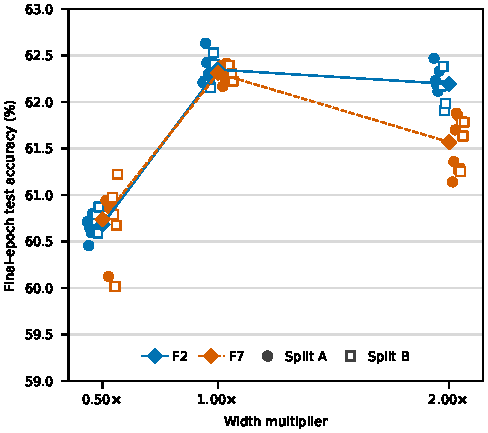
\includegraphics[width=\columnwidth]{feature_capacity_accuracy.pdf}
\xdef\xfigwd{\the\columnwidth}
\caption{Final-epoch test accuracy across the confirmatory width conditions. Each point is one split--seed record ($n=10$ per cell); circles and squares indicate Split A and Split B, respectively. Lines connect cell means. Statistical contrasts are computed from paired split--seed differences and are reported in Table~\ref{tab:confirmatory-statistics}.}
\label{fig:feature-capacity-accuracy}
\end{figure}


\subsection{Feature and Capacity Contrasts}
The complete confirmatory family is reported in
Table~\ref{tab:confirmatory-statistics}. Feature contrasts are F7 minus F2,
capacity contrasts are larger width minus smaller width, and the interaction
is the F7 capacity effect minus the F2 capacity effect. Exact two-sided
sign-permutation $p$-values are Holm-corrected across the 10 contrasts.
With $n=10$ paired split--seed units, the smallest attainable two-sided
$p$-value is $2/2^{10}=0.001953$, reported as 0.0020 when rounded.
Differences in the text and table were computed from unrounded records; the
displayed cell means are rounded.
At $2.00\times$, F7 is lower than F2 by 0.63 percentage points
(Holm-adjusted $p=0.0195$), whereas the feature contrasts at $0.50\times$
and $1.00\times$ are not distinguishable under this protocol. The
$0.50\times$--$1.00\times$ capacity increase is positive for both feature
sets, while the $1.00\times$--$2.00\times$ change is not distinguishable for
F2 and is negative for F7. The global interaction contrast is
$-0.68$ percentage points (Holm-adjusted $p=0.0312$).
The ten paired contrasts are visualized in Fig.~\ref{fig:confirmatory-test-effects}.
\begin{table*}[!t]
\caption{Post-unblind test feature--capacity contrasts. Intervals are paired $t$ 95\% intervals; raw sign-permutation $p$-values are Holm-corrected over the 10 confirmatory contrasts. Here, $d_z=\bar d/s_d$ is the standardized mean paired difference, and $n=10$ split--seed units.}
\label{tab:confirmatory-statistics}
\centering
\footnotesize
\begin{tabular*}{\textwidth}{@{\extracolsep{\fill}}ll>{\centering\arraybackslash}c>{\centering\arraybackslash}c>{\centering\arraybackslash}c>{\centering\arraybackslash}c>{\centering\arraybackslash}c l@{}}
\toprule
Contrast & Unit & Estimate (pp) & 95\% interval & $d_z$ & Raw $p$ & Holm $p$ & Decision \\
\midrule
F7--F2 at $0.50\times$ & split--seed & $+0.05$ & $[-0.23, +0.34]$ & 0.14 & 0.6738 & 1.0000 & Not distinguishable \\
F7--F2 at $1.00\times$ & split--seed & $-0.04$ & $[-0.18, +0.10]$ & $-0.21$ & 0.5137 & 1.0000 & Not distinguishable \\
F7--F2 at $2.00\times$ & split--seed & $-0.63$ & $[-0.89, -0.36]$ & $-1.71$ & 0.0020 & 0.0195 & F7 lower \\
F2: $0.50$--$2.00\times$ & split--seed & $+1.51$ & $[+1.37, +1.65]$ & 7.63 & 0.0020 & 0.0195 & Positive \\
F7: $0.50$--$2.00\times$ & split--seed & $+0.83$ & $[+0.45, +1.21]$ & 1.55 & 0.0020 & 0.0195 & Positive \\
F2: $0.50$--$1.00\times$ & split--seed & $+1.66$ & $[+1.52, +1.81]$ & 8.17 & 0.0020 & 0.0195 & Positive \\
F2: $1.00$--$2.00\times$ & split--seed & $-0.15$ & $[-0.35, +0.05]$ & $-0.55$ & 0.1055 & 0.3164 & Not distinguishable \\
F7: $0.50$--$1.00\times$ & split--seed & $+1.57$ & $[+1.28, +1.86]$ & 3.86 & 0.0020 & 0.0195 & Positive \\
F7: $1.00$--$2.00\times$ & split--seed & $-0.74$ & $[-0.97, -0.52]$ & $-2.37$ & 0.0020 & 0.0195 & Negative \\
Interaction (F7--F2 capacity effect) & split--seed & $-0.68$ & $[-1.09, -0.27]$ & $-1.18$ & 0.0078 & 0.0312 & Negative \\
\bottomrule
\end{tabular*}
\end{table*}


\begin{figure*}[!t]
\centering
\includegraphics[width=0.75\textwidth]{confirmatory_test_effects.pdf}
% The local IEEE Access class expects this width marker for ordinary figures.
\xdef\xfigwd{\the\textwidth}
\caption{Post-unblind test contrasts. Bars are paired 95\% $t$ intervals;
filled markers indicate Holm-adjusted $p<0.05$. The shaded band marks
$\pm0.15$ percentage points.}
\label{fig:confirmatory-test-effects}
\end{figure*}


\subsection{Split-Stratified Sensitivity}
Table~\ref{tab:split-sensitivity} gives split-stratified test
contrasts. The direction of the $2.00\times$ F7--F2 contrast is the same in
both splits, as is the direction of the F7 $1.00\times$--$2.00\times$
contrast. These split-specific values are descriptive consistency checks;
they are not treated as an additional independent inferential family.
\begin{table}[!t]
\caption{Split-stratified sensitivity checks for all 10 confirmatory test contrasts. These values are descriptive consistency checks, not an additional inferential family.}
\label{tab:split-sensitivity}
\centering
\footnotesize
\setlength{\tabcolsep}{3pt}
\begin{tabular*}{\columnwidth}{@{\extracolsep{\fill}}lccc@{}}
\toprule
Contrast & Split A (pp) & Split B (pp) & $n$ per split \\
\midrule
F7--F2 at 0.50$\times$ & $+0.10$ & $+0.01$ & 5 \\
F7--F2 at 1.00$\times$ & $-0.05$ & $-0.03$ & 5 \\
F7--F2 at 2.00$\times$ & $-0.68$ & $-0.58$ & 5 \\
F2: 0.50$\times$--1.00$\times$ & $+1.72$ & $+1.61$ & 5 \\
F2: 0.50$\times$--2.00$\times$ & $+1.62$ & $+1.40$ & 5 \\
F2: 1.00$\times$--2.00$\times$ & $-0.09$ & $-0.21$ & 5 \\
F7: 0.50$\times$--1.00$\times$ & $+1.57$ & $+1.57$ & 5 \\
F7: 0.50$\times$--2.00$\times$ & $+0.84$ & $+0.81$ & 5 \\
F7: 1.00$\times$--2.00$\times$ & $-0.72$ & $-0.76$ & 5 \\
Interaction (F7--F2) & $-0.78$ & $-0.59$ & 5 \\
\bottomrule
\end{tabular*}
\end{table}

The pre-unblind validation analysis gave the same contrast directions and the
same Holm decisions. It is treated as a protocol-consistency check rather than
as additional test evidence.

\section{Discussion}
\label{sec:discussion}
The post-unblind results identify a capacity effect that is concentrated in the
first width increase. From $0.50\times$ to $1.00\times$, final-epoch accuracy
increases by 1.66 percentage points for F2 and 1.57 points for F7. The next
increase is not distinguishable for F2 ($-0.15$ points), whereas F7 decreases
by 0.74 points under the same protocol. Thus, the present evidence supports a
protocol-conditional saturation pattern rather than a general claim that a
larger network is always better.

The feature contrast is not distinguishable at $0.50\times$ or $1.00\times$.
At $2.00\times$, F7 is lower than F2 by 0.63 points, and the interaction
contrast is $-0.68$ points (Holm-adjusted $p=0.0312$). These estimates answer the
declared factorial question within the tested feature ladder and width range.
They do not show that the additional channels cause noise, cannot use capacity,
or are intrinsically inferior. Such causal explanations would require further
controls beyond the present design. The standardized effects in
Table~\ref{tab:confirmatory-statistics} are likewise conditional on the
split--seed units and should not be read as device-independent performance
gains.

From a cost perspective, widening F2 from $1.00\times$ to $2.00\times$ multiplies Core
FLOPs by about 3.7 ($0.974$M to $3.586$M, Table~\ref{tab:test-cell-summary})
without a detectable accuracy gain ($-0.15$ points, 95\% interval
$[-0.35,+0.05]$). For F7, the same step reduces accuracy by 0.74 points.
Within the tested range, widening beyond $1.00\times$ therefore adds
analytical cost without a detectable gain for F2 and with a loss for F7. At a
fixed width, F7 also uses about 9\%--27\% more Core FLOPs than F2 without a
detectable benefit at $0.50\times$ or $1.00\times$. These statements concern
analytical operation counts only and do not imply latency, energy, or
edge-deployment advantages.

The split-stratified check preserves the main directions for the high-width
feature contrast and for the F7 $1.00\times$--$2.00\times$ contrast, but it is
reported descriptively rather than as a second independent inferential family.
The primary interpretation therefore remains conditional on the two declared
splits, the 128-sample observation, and the BB1 training protocol.

No Core-FLOP-matched accuracy result, SNR-region result (H4), or BB2 result
(H5) is used in the claims above. The ledger records the cost fields needed for
future matching, but the present manuscript reports nominal-width accuracy
contrasts only. This boundary prevents the unavailable analyses from being
implicitly replaced by unsupported numerical claims.

\section{Scope and Limitations}
\label{sec:limitations}
The controlled design isolates representation and capacity within a fixed
short-window setting, but its scope is intentionally bounded. The main analysis
uses one synthetic corpus, a 128-sample observation, one primary backbone, a
predefined capacity range, and a finite set of seeds and data splits. A small
secondary-backbone control is used for directional checking rather than as a
second full benchmark. The study reports parameter and operation-count costs;
it does not make a physical-device latency or energy claim. The split audit
reports the source metadata available for the corpus.

The present results use nominal width as the capacity axis. Although the cost
ledger stores Core FLOPs and can define admissible matching pairs, no
Core-FLOP-matched accuracy comparison is reported here. Likewise, the
pre-specified H4 SNR-region analysis and H5 secondary-backbone control are not
included in the current results. They should not be inferred from the nominal
width contrasts.

All widths share the same learning-rate, weight-decay, and regularization
settings. The reported capacity effects therefore describe the common protocol
and do not establish that each width was individually hyperparameter-optimal.
The nested feature ladder also changes both information content and the number
of input channels, so it does not identify which individual derived channel
causes an observed effect. Finally, the study cannot infer source-record
independence when the dataset metadata do not expose waveform provenance.
The analysis plan also specified a split-aware mixed model, but it was not fit
because only two split levels were available. The manuscript therefore uses
split-stratified descriptive checks and paired split--seed summaries instead.

\section{Data and Code Availability}
The dataset is used under its applicable research and redistribution conditions
and is not redistributed with the study records. The experimental record is
locked. The reproducibility package is available in the
feature-geometry-network-capacity-amc repository under
github.com/dogayaltinel. It contains the study source
code, split indices, cost ledger, locked aggregate analysis summaries,
environment lock, record schemas, table and figure generators, and the
manifest mapping reported quantities to their source records. The source
dataset, checkpoints, prediction arrays, and per-run training logs are not
redistributed; the dataset source and SHA-256 are recorded in the package.

\section{Conclusion}\color{black}
This paper presents a controlled short-window AMC study that separates
feature-geometry changes from network-capacity changes on a shared primary
backbone. Under the locked protocol, increasing width from $0.50\times$ to
$1.00\times$ improved final-epoch accuracy for both F2 and F7, while the
$1.00\times$--$2.00\times$ increase produced no distinguishable change for F2
and a decrease for F7. The feature contrast was not distinguishable at the two
lower widths and favored F2 at $2.00\times$; the interaction contrast was
$-0.68$ percentage points with Holm-adjusted $p=0.0312$.

These findings support a conditional conclusion about the tested feature ladder,
width range, 128-sample observation, two splits, and BB1 protocol. They do not
establish universal feature-geometry superiority, hardware latency or energy
advantages, or cross-corpus generalization. Core-FLOP-matched accuracy, SNR
region effects, and the secondary-backbone control remain outside the reported
results and are not inferred here.


\bibliographystyle{IEEEtran}
\bibliography{refs}

\color{black}
\begin{IEEEbiography}[{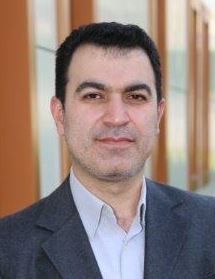
\includegraphics[width=1in,height=1.25in,clip,keepaspectratio]{dogayaltinel_medeniyet.JPG}}]{\textbf{Dogay Altinel}}
(Member, IEEE) received the B.S. degree in electronics engineering from Hacettepe University, Ankara, Turkey, in 1992, and the M.Sc. and Ph.D. degrees in telecommunications engineering from Istanbul Technical University, Istanbul, Turkey, in 2014 and 2019, respectively. From 1992 to 2012, he was in the electronics and telecommunications industry. Since 2012, he has been with Istanbul Medeniyet University, Istanbul, Turkey. His research interests include communication theory, wireless networks, energy harvesting systems, deep-learning-based communications, and applications of artificial intelligence.
\end{IEEEbiography}

\EOD
\end{document}
